%% abtex2-modelo-trabalho-academico.tex, v-1.9.6 laurocesar
%% Copyright 2012-2016 by abnTeX2 group at http://www.abntex.net.br/
%%
%% This work may be distributed and/or modified under the
%% conditions of the LaTeX Project Public License, either version 1.3
%% of this license or (at your option) any later version.
%% The latest version of this license is in
%%   http://www.latex-project.org/lppl.txt
%% and version 1.3 or later is part of all distributions of LaTeX
%% version 2005/12/01 or later.
%%
%% This work has the LPPL maintenance status `maintained'.
%%
%% The Current Maintainer of this work is the abnTeX2 team, led
%% by Lauro César Araujo. Further information are available on
%% http://www.abntex.net.br/
%%
%% This work consists of the files abntex2-modelo-trabalho-academico.tex,
%% abntex2-modelo-include-comandos and abntex2-modelo-references.bib
%%

% ------------------------------------------------------------------------
% ------------------------------------------------------------------------
% abnTeX2: Modelo de Trabalho Academico (tese de doutorado, dissertacao de
% mestrado e trabalhos monograficos em geral) em conformidade com
% ABNT NBR 14724:2011: Informacao e documentacao - Trabalhos academicos -
% Apresentacao
% ------------------------------------------------------------------------
% ------------------------------------------------------------------------

\documentclass[
	% -- opções da classe memoir --
	12pt,				% tamanho da fonte
%	openright,			% capítulos começam em pág ímpar (insere página vazia caso preciso)
%	twoside,			% para impressão em recto e verso. Oposto a oneside
    oneside,			% Oposto a twoside
	a4paper,			% tamanho do papel.
	% -- opções da classe abntex2 --
	%chapter=TITLE,		% títulos de capítulos convertidos em letras maiúsculas
	%section=TITLE,		% títulos de seções convertidos em letras maiúsculas
	%subsection=TITLE,	% títulos de subseções convertidos em letras maiúsculas
	%subsubsection=TITLE,% títulos de subsubseções convertidos em letras maiúsculas
	% -- opções do pacote babel --
	english,			% idioma adicional para hifenização
	french,				% idioma adicional para hifenização
	spanish,			% idioma adicional para hifenização
	brazil				% o último idioma é o principal do documento
	]{abntex2}

% ---
% Pacotes 
% ---
\usepackage{lmodern}			% Usa a fonte Latin Modern			
\usepackage[T1]{fontenc}		% Selecao de codigos de fonte.
\usepackage[utf8]{inputenc}		% Codificacao do documento (conversão automática dos acentos)
\usepackage{lastpage}			% Usado pela Ficha catalográfica
\usepackage{indentfirst}		% Indenta o primeiro parágrafo de cada seção.
\usepackage{color}				% Controle das cores
\usepackage{graphicx}			% Inclusão de gráficos
\usepackage{microtype} 			% para melhorias de justificação

\usepackage{lipsum}				% para geração de dummy text

\usepackage[brazilian,hyperpageref]{backref}	 % Paginas com as citações na bibl
\usepackage[alf]{abntex2cite}	% Citações padrão ABNT

% ---
% CONFIGURAÇÕES DE PACOTES
% ---

% ---
% Configurações do pacote backref
% Usado sem a opção hyperpageref de backref
\renewcommand{\backrefpagesname}{Citado na(s) página(s):~}
% Texto padrão antes do número das páginas
\renewcommand{\backref}{}
% Define os textos da citação
\renewcommand*{\backrefalt}[4]{
	\ifcase #1 %
		Nenhuma citação no texto.%
	\or
		Citado na página #2.%
	\else
		Citado #1 vezes nas páginas #2.%
	\fi}%
% ---

% ---
% Informações de dados para CAPA e FOLHA DE ROSTO
% ---
\titulo{Modelo de Trabalho \\ Final de Graduação com \abnTeX}
\autor{José da Silva}
\local{Brasil}
\data{Maio de 2016}
\orientador{João Paulo R. R. Leite}
\coorientador{Edmilson Marmo Moreira}
\instituicao{%
  Universidade Federal de Itajubá -- UNIFEI
  \par
  Instituto de Engenharia de Sistemas e Tecnologia da Informação
  \par
  Engenharia da Computação}
\tipotrabalho{Trabalho Final de Graduação}
% O preambulo deve conter o tipo do trabalho, o objetivo,
% o nome da instituição e a área de concentração
\preambulo{Monografia referente ao Trabalho Final de Graduação do curso de Engenharia da Computação da Universidade Federal de Itajubá}
% ---


% ---
% Configurações de aparência do PDF final

% alterando o aspecto da cor azul
\definecolor{blue}{RGB}{41,5,195}

% informações do PDF
\makeatletter
\hypersetup{
     	%pagebackref=true,
		pdftitle={\@title},
		pdfauthor={\@author},
    	pdfsubject={\imprimirpreambulo},
	    pdfcreator={LaTeX with abnTeX2},
		pdfkeywords={abnt}{latex}{abntex}{abntex2}{trabalho acadêmico},
		colorlinks=true,       		% false: boxed links; true: colored links
    	linkcolor=blue,          	% color of internal links
    	citecolor=blue,        		% color of links to bibliography
    	filecolor=magenta,      		% color of file links
		urlcolor=blue,
		bookmarksdepth=4
}
\makeatother
% ---

% ---
% Espaçamentos entre linhas e parágrafos
% ---

% O tamanho do parágrafo é dado por:
\setlength{\parindent}{1.3cm}

% Controle do espaçamento entre um parágrafo e outro:
\setlength{\parskip}{0.2cm}  % tente também \onelineskip

% ---
% compila o indice
% ---
\makeindex
% ---

% ----
% Início do documento
% ----
\begin{document}

% Seleciona o idioma do documento (conforme pacotes do babel)
%\selectlanguage{english}
\selectlanguage{brazil}

% Retira espaço extra obsoleto entre as frases.
\frenchspacing

% ----------------------------------------------------------
% ELEMENTOS PRÉ-TEXTUAIS
% ----------------------------------------------------------
% Capa e Folha de Rosto
\imprimircapa
\imprimirfolhaderosto*
% ---

% ---
% Dedicatória
% ---
\begin{dedicatoria}
   \vspace*{\fill}
   \centering
   \noindent
   \textit{ Este trabalho é dedicado às crianças adultas que,\\
   quando pequenas, sonharam em se tornar cientistas.} \vspace*{\fill}
\end{dedicatoria}
% ---

% ---
% Agradecimentos
% ---
\begin{agradecimentos}
Lorem ipsum dolor sit amet, consectetur adipiscing elit. Mauris est ipsum, lobortis vehicula scelerisque et, consequat in urna. Mauris aliquet placerat ex. Ut vel erat nisi. Nam in nisl pellentesque, tincidunt enim ut, efficitur justo. Vestibulum ante ipsum primis in faucibus orci luctus et ultrices posuere cubilia Curae; Duis id nulla consectetur, suscipit nisi sit amet, ornare lectus. Fusce fermentum, urna ac commodo varius, lectus ipsum commodo nulla, sit amet lacinia ipsum neque eget sem. Nunc pulvinar eros lectus, sit amet ornare metus semper vitae.

Sed dapibus metus sed velit vehicula, ac aliquet lorem lobortis. Nam nec elit justo. Morbi sollicitudin est mollis, rutrum sapien sed, luctus nisl. Praesent dignissim a dui quis finibus. Vestibulum sodales venenatis metus. Nulla lacinia elit sit amet iaculis congue. Proin pellentesque in orci laoreet blandit.
\end{agradecimentos}
% ---

% ---
% Epígrafe
% ---
\begin{epigrafe}
    \vspace*{\fill}
	\begin{flushright}
		\textit{``Não vos amoldeis às estruturas deste mundo, \\
		mas transformai-vos pela renovação da mente, \\
		a fim de distinguir qual é a vontade de Deus: \\
		o que é bom, o que Lhe é agradável, o que é perfeito.\\
		(Bíblia Sagrada, Romanos 12, 2)}
	\end{flushright}
\end{epigrafe}
% ---

% ---
% RESUMOS
% ---

% resumo em português
\setlength{\absparsep}{18pt} % ajusta o espaçamento dos parágrafos do resumo
\begin{resumo}
 Segundo a \citeonline[3.1-3.2]{NBR6028:2003}, o resumo deve ressaltar o
 objetivo, o método, os resultados e as conclusões do documento. A ordem e a extensão
 destes itens dependem do tipo de resumo (informativo ou indicativo) e do
 tratamento que cada item recebe no documento original. O resumo deve ser
 precedido da referência do documento, com exceção do resumo inserido no
 próprio documento. (\ldots) As palavras-chave devem figurar logo abaixo do
 resumo, antecedidas da expressão Palavras-chave:, separadas entre si por
 ponto e finalizadas também por ponto.

 \textbf{Palavras-chave}: latex. abntex. editoração de texto.
\end{resumo}

% resumo em inglês
\begin{resumo}[Abstract]
 \begin{otherlanguage*}{english}
   This is the english abstract.

   \vspace{\onelineskip}

   \noindent
   \textbf{Keywords}: latex. abntex. text editoration.
 \end{otherlanguage*}
\end{resumo}

% ---
% inserir lista de ilustrações
% ---
\pdfbookmark[0]{\listfigurename}{lof}
\listoffigures*
\clearpage
% ---

% ---
% inserir lista de tabelas
% ---
\pdfbookmark[0]{\listtablename}{lot}
\listoftables*
\clearpage
% ---

% ---
% inserir lista de abreviaturas e siglas
% ---
\begin{siglas}
  \item[ABNT] Associação Brasileira de Normas Técnicas
  \item[abnTeX] ABsurdas Normas para TeX
\end{siglas}
% ---

% ---
% inserir o sumario
% ---
\pdfbookmark[0]{\contentsname}{toc}
\tableofcontents*
\clearpage
% ---

% ----------------------------------------------------------
% ELEMENTOS TEXTUAIS
% ----------------------------------------------------------
\textual

% ----------------------------------------------------------------
% Introdução e Conceitos Básicos *******************
% ----------------------------------------------------------------
\chapter{Introdução}

\section{Como Estruturar o Projeto de Pesquisa}

Pode-se definir pesquisa como o procedimento racional e sistemático
que tem como objetivo proporcionar respostas aos problemas que são
propostos. A pesquisa é requerida quando não se dispõe de informação
suficiente para responder ao pro\-blema, ou então quando a
informação disponível se encontra em tal estado de desordem que não
possa ser adequadamente relacionada ao problema \cite{Gil}.

A pesquisa é desenvolvida mediante o concurso dos conhecimentos
disponíveis e a utilização cuidadosa de métodos, técnicas e outros
procedimentos científicos. Na realidade, a pesquisa desenvolve-se
ao longo de um processo que envolve inúmeras fases, desde a
adequada formulação ao problema até a satisfatória apresentação
dos resultados.

A pesquisa é classificada como científica quando satisfaz a
determinadas condi\-ções. Seu objeto deve ser  perfeitamente
definido de forma que possa ser reconhecível e identificável por
todos. O estudo deve acrescentar algo ao que já se sabe sobre o
assunto e ser útil como fonte de pesquisa, fornecendo elementos que
permitam a verificação e a contestação das hipóteses apresentadas,
tendo em vista a sua continuidade.

O projeto é uma das etapas componentes do processo de elaboração,
execução e apresentação da pesquisa. Esta necessita ser planejada
com extremo rigor, caso contrário o investigador, em determinada
altura, encontrar-se-á perdido num emaranhado de dados colhidos, sem
saber como dispor dos mesmos ou até desconhecendo seu significado e
importância \cite{Marconi}.

Em uma pesquisa, nada se faz ao acaso. Desde a escolha do tema,
fixação dos objetivos, determinação da metodologia, coleta dos
dados, sua análise e interpretação para a elaboração do relatório
final, tudo é previsto no projeto de pesquisa.


\section{Elementos de Um Projeto de Pesquisa}

Não há, evidentemente, regras fixas acerca da elaboração de um
projeto. Sua estrutura é determinada pelo tipo de problema a ser
pesquisado e também pelo estilo de seus autores. É necessário que o
projeto esclareça como se processará a pesquisa, quais as etapas que
serão desenvolvidas e quais os recursos que devem ser alocados para
atingir seus objetivos. É necessário, também, que o projeto seja
suficientemente detalhado para proporcionar a avaliação do processo
de pesquisa \cite{Gil}.

Os elementos habitualmente requeridos num projeto são os seguintes
\cite{Marconi}:

\begin{enumerate}
    \item Apresentação.
    \item Objetivo.
    \item Justificativa.
    \item Objeto.
    \item Metodologia.
    \item Embasamento Teórico.
    \item Cronograma.
    \item Bibliografia.
\end{enumerate}

\subsection{Apresentação}

A apresentação do projeto de pesquisa responde à questão
\emph{quem?}, ou seja, apresenta o(s) autor(es), coordenador,
título do trabalho, local etc.

É importante ressaltar que o título difere do tema. Enquanto este
último sofre um processo de delimitação e especificação, para
torná-lo viável à realização da pesquisa, o título sintetiza o
conteúdo da mesma.

Portanto, o título de uma pesquisa não corresponde ao \emph{tema},
nem à \emph{delimitação do tema}, mas emana dos \emph{objetivos
geral e específicos}, quase como uma síntese dos mesmos.

\subsection{Objetivo}

A especificação do objetivo de uma pesquisa responde questões
\emph{para quê?} e \emph{para quem?} Apresenta:

\begin{description}
    \item[Tema:] É o assunto que se deseja provar ou
    desenvolver. O tema é, nessa fase, necessariamente amplo,
    precisando bem o assunto geral sobre o qual se deseja realizar
    a pesquisa.

    \item[Delimitação do Tema:] O processo de delimitação do tema
    só é dado por concluído quando se faz a limitação geográfica e
    espacial do mesmo, com vistas a realização da pesquisa.

    \item[Objetivo Geral:] Está ligado a uma visão global e
    abrangente do tema. Relaciona-se com o conteúdo intrínseco,
    quer dos fenômenos e eventos, quer das idéias estudadas.
    Vincula-se diretamente à própria significação da tese proposta
    pelo projeto.

    \item[Objetivos Específicos:] Apresentam caráter mais concreto.
    Têm função intermediária e instrumental, permitindo, de um
    lado, atingir o objetivo geral e, de outro, aplicar este a
    situações particulares.
\end{description}

\subsection{Justificativa}

É o único item do projeto que apresenta respostas à questão
\emph{por quê?} Consiste numa exposição sucinta, porém completa,
das razões de ordem teórica e dos motivos de ordem prática que
tornam importante a realização da pesquisa. Deve enfatizar:

\begin{itemize}
    \item o estágio em que se encontra a teoria respeitante ao
    tema;

    \item as contribuições teóricas a pesquisa pode trazer:
    \begin{itemize}
        \item confirmação geral;

        \item confirmação na sociedade particular em que se insere
        a pesquisa;

        \item especificação para casos particulares;

        \item clarificação da teoria;

        \item resolução de pontos obscuros etc.
    \end{itemize}

    \item importância do tema do ponto de vista geral;

    \item importância do tema para os casos particulares em
    questão;

    \item possibilidade de sugerir modificações no âmbito da
    realidade abarcada pelo tema proposto;

    \item descoberta de soluções para casos gerais e/ou
    particulares etc.
\end{itemize}

A justificativa difere da revisão bibliográfica e, por este
motivo, não apresenta citações de outros autores. Difere, também,
da teoria de base, que vai servir de elemento unificador entre o
concreto da pesquisa e o conhecimento teórico da ciência na qual
se insere. Portanto, quando se trata de analisar as razões de
ordem teórica ou se referir ao estágio de desenvolvimento da
teoria pretende-se apenas ressaltar a importância da pesquisa no
campo da teoria.

Deduz-se, dessas características, que ao conhecimento científico
do pesquisador soma-se boa parte de criatividade e capacidade de
convencer, para a redação da justificativa.

\subsection{Objeto}

Responde à pergunta \emph{o quê?}, o objeto da pesquisa engloba:

\begin{description}
    \item[Problema:] A formulação do problema prende-se ao tema
    proposto: ela esclarece a dificuldade específica com a qual se
    defronta e que se pretende resolver por intermédio da
    pesquisa.

    \item[Hipótese Básica:] O ponto básico do tema, individualizado
    e especificado na formulação do problema, sendo uma
    dificuldade sentida, compreendida e definida, necessita de uma
    resposta, ``provável, suposta e provisória'', isto é, uma
    hipótese.

    \item[Hipóteses Secundárias:] São afirmações (toda hipótese é
    uma afirmação) complementares da básica.
\end{description}

\subsection{Metodologia}

A especificação da metodologia da pesquisa é a que abrange maior
número de itens, pois responde, a um só tempo, às questões
\emph{como?, com quê?, onde?, quanto?} Corresponde a componentes
como:

\begin{description}
    \item[Método de Abordagem:] O método se caracteriza por uma
    abordagem mais ampla, em nível de abstração mais elevado, dos
    fenômenos da natureza e da sociedade.
    \item[Métodos de Procedimento:] Constituem etapas mais
    concretas da investigação, com finalidade mais restrita em
    termos de explicação geral dos fenômenos menos abstratos.
    Pressupõem uma atitude concreta em relação ao fenômeno e estão
    limitadas a um domínio particular.
    \item[Técnicas:] São consideradas um conjunto de preceitos ou
    processos de que se serve uma ciência; são, também, a
    habilidade para usar esses preceitos ou normas, na obtenção de
    seus propósitos. Correspondem, portanto, à parte prática de
    coleta de dados.
\end{description}

\subsection{Embasamento Teórico}

Responde ainda à questão \emph{como?}, aparecem aqui os elementos
de fundamentação teórica da pesquisa e, também, a definição dos
conceitos empregados.

É no embasamento teórico que se situa a revisão bibliográfica.
Entretanto, para atender a primeira fase do TD a revisão
bibliográfica não é uma exigência, uma vez que deverá ser
apresentada na segunda fase do trabalho.

\subsection{Cronograma}

A elaboração do cronograma responde à pergunta \emph{quando?} A
pesquisa deve ser dividida em partes, fazendo-se a previsão do
tempo necessário para passar de uma fase a outra.

\subsection{Bibliografia}

A bibliografia final, apresentada no projeto de pesquisa, abrange
os livros, artigos, publicações e documentos utilizados, nas
diferentes fases.


\section{Normas Para Elaboração do Projeto}

A redação do projeto, assim como as demais monografias apresentadas
durante o desenvolvimento do TD, deverá estar no padrão da
Associação Brasileira de Normas Técnicas (ABNT), adequada à normas
elaboradas pela coordenação do TD do curso de Engenharia da
Computação da Universidade Federal de Itajubá.

% ----------------------------------------------------------------
% Introdução e Conceitos Básicos *******************
% ----------------------------------------------------------------
\chapter{Revisão Bibliográfica}

\section{Lorem Ipsum - Part I}

Interdum et malesuada fames ac ante ipsum primis in faucibus. Nullam varius dui nec ligula facilisis, in condimentum ante aliquet. Aliquam luctus quam sit amet risus dictum, eu iaculis dui tristique. Cras egestas ante non elementum porta. Suspendisse potenti. Nam tristique et libero vel dapibus. Vestibulum ante ipsum primis in faucibus orci luctus et ultrices posuere cubilia Curae; Cras massa est, iaculis nec imperdiet eu, cursus et ipsum. Vestibulum accumsan erat ac placerat semper. Quisque volutpat tempor ornare.

Nunc eu suscipit lectus. Maecenas suscipit tellus eu nisi rhoncus iaculis. Sed vel massa sit amet est posuere vulputate vitae ac lorem. Etiam hendrerit odio sed nunc varius dictum. Vestibulum varius turpis at luctus feugiat. Cras ante massa, dapibus a tellus ut, iaculis ultricies enim. Morbi sollicitudin bibendum leo eu auctor. Aliquam a quam ornare, fringilla augue vel, pretium felis. Ut quis nunc placerat, varius arcu ac, iaculis lectus. Nunc neque ex, malesuada id justo quis, iaculis hendrerit magna. Vestibulum eu ipsum non leo eleifend efficitur. Nunc sodales rutrum metus, ut hendrerit mauris dignissim non. Vivamus nec turpis ut sapien vestibulum sagittis. Donec venenatis metus non finibus fringilla. Praesent maximus sapien sit amet mi vestibulum, sit amet euismod tortor dignissim. Vestibulum et ante ut mi egestas viverra consequat consequat nisi.

Vivamus odio ex, gravida eget dignissim quis, euismod vitae nulla. Curabitur in leo non nulla molestie laoreet feugiat ut nunc. Mauris laoreet quam a ligula semper scelerisque. Maecenas porttitor erat sem, imperdiet ultricies neque semper id. Integer aliquet nibh libero, sit amet pulvinar ipsum rhoncus ac. Nullam interdum libero non ex varius, quis rhoncus ex feugiat. Quisque nec est a augue elementum facilisis sit amet a purus. Proin vel lacus tristique, luctus nunc a, convallis tellus. Maecenas lobortis ornare dapibus. Class aptent taciti sociosqu ad litora torquent per conubia nostra, per inceptos himenaeos.


\section{Lorem Ipsum - Part II}

Lorem ipsum dolor sit amet, consectetur adipiscing elit. Mauris est ipsum, lobortis vehicula scelerisque et, consequat in urna. Mauris aliquet placerat ex. Ut vel erat nisi. Nam in nisl pellentesque, tincidunt enim ut, efficitur justo. Vestibulum ante ipsum primis in faucibus orci luctus et ultrices posuere cubilia Curae; Duis id nulla consectetur, suscipit nisi sit amet, ornare lectus. Fusce fermentum, urna ac commodo varius, lectus ipsum commodo nulla, sit amet lacinia ipsum neque eget sem. Nunc pulvinar eros lectus, sit amet ornare metus semper vitae.

Sed dapibus metus sed velit vehicula, ac aliquet lorem lobortis. Nam nec elit justo. Morbi sollicitudin est mollis, rutrum sapien sed, luctus nisl. Praesent dignissim a dui quis finibus. Vestibulum sodales venenatis metus. Nulla lacinia elit sit amet iaculis congue. Proin pellentesque in orci laoreet blandit.

% ----------------------------------------------------------------
% Metodologia *******************
% ----------------------------------------------------------------
\chapter{Metodologia}

\section{Lorem Ipsum - Part I}

Interdum et malesuada fames ac ante ipsum primis in faucibus. Nullam varius dui nec ligula facilisis, in condimentum ante aliquet. Aliquam luctus quam sit amet risus dictum, eu iaculis dui tristique. Cras egestas ante non elementum porta. Suspendisse potenti. Nam tristique et libero vel dapibus. Vestibulum ante ipsum primis in faucibus orci luctus et ultrices posuere cubilia Curae; Cras massa est, iaculis nec imperdiet eu, cursus et ipsum. Vestibulum accumsan erat ac placerat semper. Quisque volutpat tempor ornare.

Nunc eu suscipit lectus. Maecenas suscipit tellus eu nisi rhoncus iaculis. Sed vel massa sit amet est posuere vulputate vitae ac lorem. Etiam hendrerit odio sed nunc varius dictum. Vestibulum varius turpis at luctus feugiat. Cras ante massa, dapibus a tellus ut, iaculis ultricies enim. Morbi sollicitudin bibendum leo eu auctor. Aliquam a quam ornare, fringilla augue vel, pretium felis. Ut quis nunc placerat, varius arcu ac, iaculis lectus. Nunc neque ex, malesuada id justo quis, iaculis hendrerit magna. Vestibulum eu ipsum non leo eleifend efficitur. Nunc sodales rutrum metus, ut hendrerit mauris dignissim non. Vivamus nec turpis ut sapien vestibulum sagittis. Donec venenatis metus non finibus fringilla. Praesent maximus sapien sit amet mi vestibulum, sit amet euismod tortor dignissim. Vestibulum et ante ut mi egestas viverra consequat consequat nisi.

Vivamus odio ex, gravida eget dignissim quis, euismod vitae nulla. Curabitur in leo non nulla molestie laoreet feugiat ut nunc. Mauris laoreet quam a ligula semper scelerisque. Maecenas porttitor erat sem, imperdiet ultricies neque semper id. Integer aliquet nibh libero, sit amet pulvinar ipsum rhoncus ac. Nullam interdum libero non ex varius, quis rhoncus ex feugiat. Quisque nec est a augue elementum facilisis sit amet a purus. Proin vel lacus tristique, luctus nunc a, convallis tellus. Maecenas lobortis ornare dapibus. Class aptent taciti sociosqu ad litora torquent per conubia nostra, per inceptos himenaeos.


\section{Lorem Ipsum - Part II}

Lorem ipsum dolor sit amet, consectetur adipiscing elit. Mauris est ipsum, lobortis vehicula scelerisque et, consequat in urna. Mauris aliquet placerat ex. Ut vel erat nisi. Nam in nisl pellentesque, tincidunt enim ut, efficitur justo. Vestibulum ante ipsum primis in faucibus orci luctus et ultrices posuere cubilia Curae; Duis id nulla consectetur, suscipit nisi sit amet, ornare lectus. Fusce fermentum, urna ac commodo varius, lectus ipsum commodo nulla, sit amet lacinia ipsum neque eget sem. Nunc pulvinar eros lectus, sit amet ornare metus semper vitae.

Sed dapibus metus sed velit vehicula, ac aliquet lorem lobortis. Nam nec elit justo. Morbi sollicitudin est mollis, rutrum sapien sed, luctus nisl. Praesent dignissim a dui quis finibus. Vestibulum sodales venenatis metus. Nulla lacinia elit sit amet iaculis congue. Proin pellentesque in orci laoreet blandit.

\begin{figure}[!ht]
  \centering
  % Requires \usepackage{graphicx}
  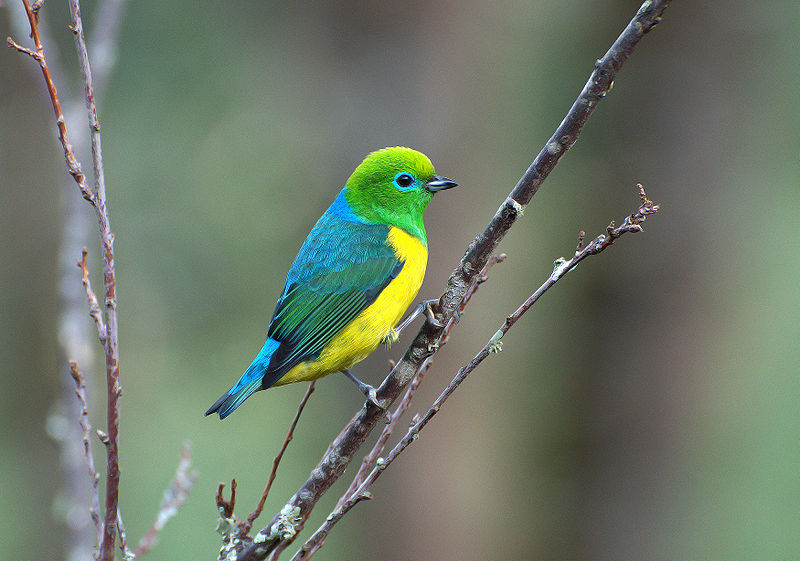
\includegraphics[width=300pt]{abntex2-modelo-livro-bandeirinha.jpg}\\
  \caption{Figura Meramente Ilustrativa}\label{fig1}
\end{figure}

% ----------------------------------------------------------------
% Experimentos e Resultados *******************
% ----------------------------------------------------------------
\chapter{Experimentos e Resultados}

\section{Lorem Ipsum - Part I}

Interdum et malesuada fames ac ante ipsum primis in faucibus. Nullam varius dui nec ligula facilisis, in condimentum ante aliquet. Aliquam luctus quam sit amet risus dictum, eu iaculis dui tristique. Cras egestas ante non elementum porta. Suspendisse potenti. Nam tristique et libero vel dapibus. Vestibulum ante ipsum primis in faucibus orci luctus et ultrices posuere cubilia Curae; Cras massa est, iaculis nec imperdiet eu, cursus et ipsum. Vestibulum accumsan erat ac placerat semper. Quisque volutpat tempor ornare.

Nunc eu suscipit lectus. Maecenas suscipit tellus eu nisi rhoncus iaculis. Sed vel massa sit amet est posuere vulputate vitae ac lorem. Etiam hendrerit odio sed nunc varius dictum. Vestibulum varius turpis at luctus feugiat. Cras ante massa, dapibus a tellus ut, iaculis ultricies enim. Morbi sollicitudin bibendum leo eu auctor. Aliquam a quam ornare, fringilla augue vel, pretium felis. Ut quis nunc placerat, varius arcu ac, iaculis lectus. Nunc neque ex, malesuada id justo quis, iaculis hendrerit magna. Vestibulum eu ipsum non leo eleifend efficitur. Nunc sodales rutrum metus, ut hendrerit mauris dignissim non. Vivamus nec turpis ut sapien vestibulum sagittis. Donec venenatis metus non finibus fringilla. Praesent maximus sapien sit amet mi vestibulum, sit amet euismod tortor dignissim. Vestibulum et ante ut mi egestas viverra consequat consequat nisi.

Vivamus odio ex, gravida eget dignissim quis, euismod vitae nulla. Curabitur in leo non nulla molestie laoreet feugiat ut nunc. Mauris laoreet quam a ligula semper scelerisque. Maecenas porttitor erat sem, imperdiet ultricies neque semper id. Integer aliquet nibh libero, sit amet pulvinar ipsum rhoncus ac. Nullam interdum libero non ex varius, quis rhoncus ex feugiat. Quisque nec est a augue elementum facilisis sit amet a purus. Proin vel lacus tristique, luctus nunc a, convallis tellus. Maecenas lobortis ornare dapibus. Class aptent taciti sociosqu ad litora torquent per conubia nostra, per inceptos himenaeos.


\section{Lorem Ipsum - Part II}

Lorem ipsum dolor sit amet, consectetur adipiscing elit. Mauris est ipsum, lobortis vehicula scelerisque et, consequat in urna. Mauris aliquet placerat ex. Ut vel erat nisi. Nam in nisl pellentesque, tincidunt enim ut, efficitur justo. Vestibulum ante ipsum primis in faucibus orci luctus et ultrices posuere cubilia Curae; Duis id nulla consectetur, suscipit nisi sit amet, ornare lectus. Fusce fermentum, urna ac commodo varius, lectus ipsum commodo nulla, sit amet lacinia ipsum neque eget sem. Nunc pulvinar eros lectus, sit amet ornare metus semper vitae.

Sed dapibus metus sed velit vehicula, ac aliquet lorem lobortis. Nam nec elit justo. Morbi sollicitudin est mollis, rutrum sapien sed, luctus nisl. Praesent dignissim a dui quis finibus. Vestibulum sodales venenatis metus. Nulla lacinia elit sit amet iaculis congue. Proin pellentesque in orci laoreet blandit.

\begin{table}[h]
    \begin{center}    
    \begin{tabular}{ | l | l | l | p{5cm} |}
    \hline
    Day & Min Temp & Max Temp & Summary \\ \hline
    Monday & 11C & 22C & A clear day with lots of sunshine.
    However, the strong breeze will bring down the temperatures. \\ \hline
    Tuesday & 9C & 19C & Cloudy with rain, across many northern regions. Clear spells
    across most of Scotland and Northern Ireland,
    but rain reaching the far northwest. \\ \hline
    Wednesday & 10C & 21C & Rain will still linger for the morning.
    Conditions will improve by early afternoon and continue
    throughout the evening. \\
    \hline
    \end{tabular}
    \caption[Tabela Ilustrativa]{Tabela Ilustrativa }
    \label{tab1}
    \end{center}
\end{table}


% ----------------------------------------------------------------
% Conclusão e Trabalhos Futuros *******************
% ----------------------------------------------------------------
\chapter{Conclusão}

\section{Lorem Ipsum - Part I}

Interdum et malesuada fames ac ante ipsum primis in faucibus. Nullam varius dui nec ligula facilisis, in condimentum ante aliquet. Aliquam luctus quam sit amet risus dictum, eu iaculis dui tristique. Cras egestas ante non elementum porta. Suspendisse potenti. Nam tristique et libero vel dapibus. Vestibulum ante ipsum primis in faucibus orci luctus et ultrices posuere cubilia Curae; Cras massa est, iaculis nec imperdiet eu, cursus et ipsum. Vestibulum accumsan erat ac placerat semper. Quisque volutpat tempor ornare.

Nunc eu suscipit lectus. Maecenas suscipit tellus eu nisi rhoncus iaculis. Sed vel massa sit amet est posuere vulputate vitae ac lorem. Etiam hendrerit odio sed nunc varius dictum. Vestibulum varius turpis at luctus feugiat. Cras ante massa, dapibus a tellus ut, iaculis ultricies enim. Morbi sollicitudin bibendum leo eu auctor. Aliquam a quam ornare, fringilla augue vel, pretium felis. Ut quis nunc placerat, varius arcu ac, iaculis lectus. Nunc neque ex, malesuada id justo quis, iaculis hendrerit magna. Vestibulum eu ipsum non leo eleifend efficitur. Nunc sodales rutrum metus, ut hendrerit mauris dignissim non. Vivamus nec turpis ut sapien vestibulum sagittis. Donec venenatis metus non finibus fringilla. Praesent maximus sapien sit amet mi vestibulum, sit amet euismod tortor dignissim. Vestibulum et ante ut mi egestas viverra consequat consequat nisi.

Vivamus odio ex, gravida eget dignissim quis, euismod vitae nulla. Curabitur in leo non nulla molestie laoreet feugiat ut nunc. Mauris laoreet quam a ligula semper scelerisque. Maecenas porttitor erat sem, imperdiet ultricies neque semper id. Integer aliquet nibh libero, sit amet pulvinar ipsum rhoncus ac. Nullam interdum libero non ex varius, quis rhoncus ex feugiat. Quisque nec est a augue elementum facilisis sit amet a purus. Proin vel lacus tristique, luctus nunc a, convallis tellus. Maecenas lobortis ornare dapibus. Class aptent taciti sociosqu ad litora torquent per conubia nostra, per inceptos himenaeos.


\section{Lorem Ipsum - Part II}

Lorem ipsum dolor sit amet, consectetur adipiscing elit. Mauris est ipsum, lobortis vehicula scelerisque et, consequat in urna. Mauris aliquet placerat ex. Ut vel erat nisi. Nam in nisl pellentesque, tincidunt enim ut, efficitur justo. Vestibulum ante ipsum primis in faucibus orci luctus et ultrices posuere cubilia Curae; Duis id nulla consectetur, suscipit nisi sit amet, ornare lectus. Fusce fermentum, urna ac commodo varius, lectus ipsum commodo nulla, sit amet lacinia ipsum neque eget sem. Nunc pulvinar eros lectus, sit amet ornare metus semper vitae.

Sed dapibus metus sed velit vehicula, ac aliquet lorem lobortis. Nam nec elit justo. Morbi sollicitudin est mollis, rutrum sapien sed, luctus nisl. Praesent dignissim a dui quis finibus. Vestibulum sodales venenatis metus. Nulla lacinia elit sit amet iaculis congue. Proin pellentesque in orci laoreet blandit.


% ----------------------------------------------------------
% ELEMENTOS PÓS-TEXTUAIS
% ----------------------------------------------------------
\postextual
% ----------------------------------------------------------

% ----------------------------------------------------------
% Referências bibliográficas
% ----------------------------------------------------------
\bibliography{abntex2-modelo-references}

% ----------------------------------------------------------
% Glossário
% ----------------------------------------------------------
%
% Consulte o manual da classe abntex2 para orientações sobre o glossário.
%
%\glossary

% ----------------------------------------------------------
% Apêndices
% ----------------------------------------------------------

% ---
% Inicia os apêndices
% ---
\begin{apendicesenv}

% Imprime uma página indicando o início dos apêndices
\partapendices
% ----------------------------------------------------------
\chapter{Quisque libero justo}
% ----------------------------------------------------------
\lipsum[50]

\end{apendicesenv}
% ---



\end{document}
